\chapter{Lec 18 - Long-Term Dependencies}

\section{Learning Long-Term Dependencies}
The basic problem of learning long-term dependencies is that gradients propagated over many stages tend to either vanish (most of the time) or explode\footnote{a problem when large error gradients accumulate and result in very large updates to neural network model weights during training} (rarely, but with much damage to the optimization).\newline\newline
A long-term dependency is when the desired output at time $t$ depends on the input at time $t - \tau$, with $t > \tau >> 1$ (e.g. $\textbf{x}^{(t - 100)} \rightarrow \textbf{y}^{(t)}$).\newline\newline
This means that, for the Recurrent Neural Network to output the correct
desired $\textbf{y}^{(t)}$, it has to recognize its dependency on $\textbf{x}^{(t - \tau)}$, and use $\textbf{x}^{(t - \tau)}$ in the generation of $\textbf{y}^{(t)}$.
\newline\newline
Here are some approaches to try to reduce the vanishing/exploding gradients
problem:
\begin{itemize}
    \item Architectural
    \begin{itemize}
        \item Long Short-Term Memory or Gated Recurrent units
        \item Reservoir Computing: Echo State Networks and Liquid State Machines
    \end{itemize}
    \item Algorithmic
    \begin{itemize}
        \item Clipping gradients (avoids exploding gradients)
        \item Hessian Free Optimization
        \item Smart Initialization: pre-training techniques
    \end{itemize}
\end{itemize}

\section{Long Short-Term Memory}
Long Short Term Memory networks - usually just called “LSTMs” - are a special kind of RNN, capable of learning long-term dependencies.\newline\newline
They are based on the idea of creating paths through time that have derivatives that neither vanish nor explode.\newline\newline
The mechanism allows the networks to “remember” relevant information for a long period of time and to "forget" them when they are no more relevant.
\newline\newline
The LSTM does have the ability to remove or add information to the cell state, carefully regulated by structures called gates. Gates are a way to optionally let information through. They are composed out of a sigmoid neural net layer and a pointwise multiplication operation. The sigmoid layer outputs numbers between zero and one, describing how much of each component should be let through. A value of zero means “let nothing through,” while a value of one means “let 
verything through!”
\newline\newline
An LSTM has three of these gates, to protect and control the cell state:
\begin{enumerate}
    \item Forget gate: The sigmoid layer called the “forget gate layer ”\textit{decides} what information we’re going to throw away from the cell state. It looks at $h^{(t-1)}$ and $x^{(t)}$, and outputs a number between 0 and 1 for each number in the cell state $C^{(t-1)}$ . A 1 represents “completely keep this” while a 0 represents “completely get rid of this.” Let $f_t$ be its output. The forget gate multiplies the old state by $f_t$, forgetting the things it decided to forget.
    \begin{center}
        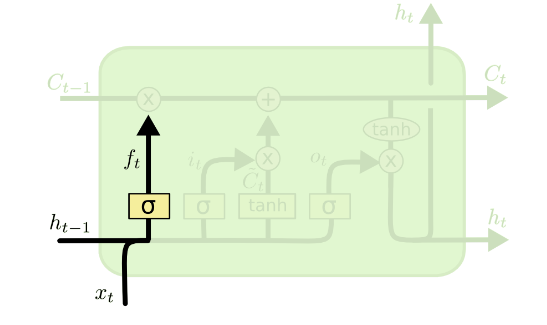
\includegraphics[]{images/forget-gate.png}
    \end{center}

    \item Input gate: It decides what new information are going to be stored in the cell state. This has two parts. First, a sigmoid layer called the “input gate layer” decides which values are going to be updated. Let $i^t$ be its output. Next, a tanh layer creates a vector of new candidate values, $\Tilde{C^t}$, that could be added to the state. The input gate computes $i^t * \Tilde{C^t}$. The output of this gate is added to the output of the forget gate to determine the new cell state.
    \begin{center}
        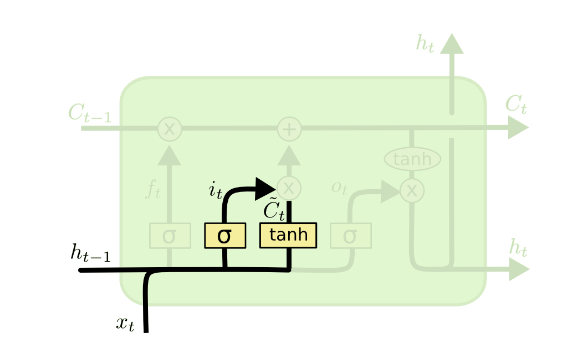
\includegraphics[]{images/Input-gate.png}
        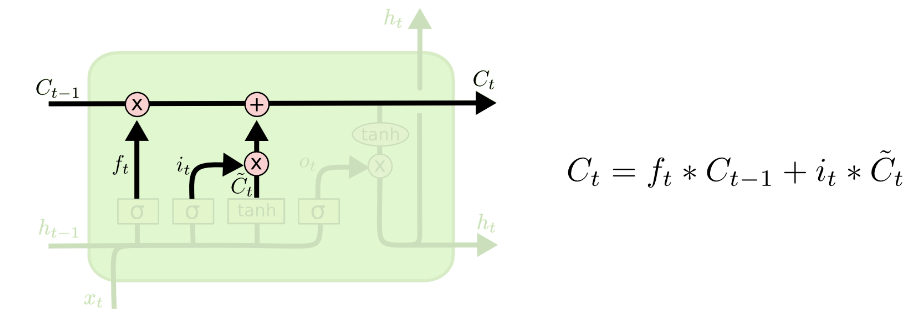
\includegraphics[scale=0.9]{images/new cell-state.png}
    \end{center}
    
    \item Output gate: It deterines what parts of the cell state are going to be outputted. It puts the cell state through tanh (to push the values to be between -1 and 1). The result is multiplied by the output of a sigmoid layer so that it only outputs the parts it decided to.
    \begin{center}
        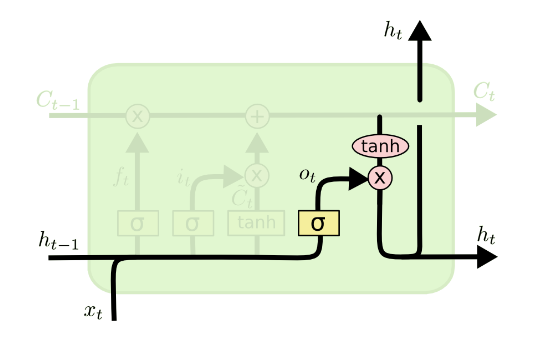
\includegraphics[]{images/output-gate.png}
    \end{center}
\end{enumerate}
There are a lot of variations of the LSTM architecture. One popular variant is adding “peephole connections.” This means that we let the gate layers look at the cell state. Other variations are:
\begin{itemize}
    \item No Input Gate (NIG)
    \item No Forget Gate (NFG)
    \item No Output Gate (NOG)
    \item No Input Activation Function (NIAF)
    \item No Output Activation Function (NOAF)
\end{itemize}
However, vanilla LSTM performs reasonably well in general and variations do not significantly improve the performance. Furthermore, the forget gate is crucial for LSTM performance.

\section{Simplifying LSTM: Gated Recurrent Units}
The main difference between GRU and LSTM is that GRU uses a single gating unit that simultaneously controls the forgetting factor and the decision to update the state unit.
\begin{center}
    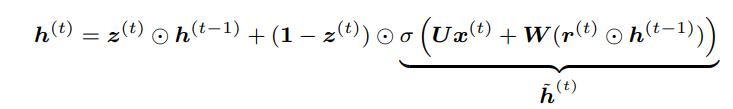
\includegraphics[]{images/GRU.png}
\end{center}
The update gate $\textbf{z}$ selects whether the hidden state need to be updated with a new hidden state $\Tilde{\textbf{h}}$. The reset gate $\textbf{r}$ decides whether the previous hidden state is ignored.\newline\newline
The values for $\textbf{z}$ and $\textbf{r}$ are defined as usual using the sigmoidal layers as in LSTM.\newline\newline
Basically, the idea is that if the $\textbf{z}$ vector has a value equal to 0 in position $i$, when we compute the element-wise multiplication between $\textbf{z}$ and $\textbf{h}^{(t-1)}$ the $i$-th value in $\textbf{h}^{(t-1)}$ will be cancelled. On the other hand, the $i$-th element in $(1 - \textbf{z})$ is 1. Therefore, the $i$-th element of $\textbf{h}^{(t-1)}$ will be updated with the $i$-th element of $\Tilde{\textbf{h}}$.

\section{Reservoir Computing}
Reservoir Computing is an umbrella term used to identify a general framework of computation derived from Recurrent Neural Networks (RNN). This technique can be implemented with \textbf{Echo State Networks} and \textbf{Liquid State Machines}. The idea is to fix the input-to-hidden and hidden-to-hidden connections at random values and only learn the output units connections. The intuition was born from the fact that in training RNNs most of the times the weights showing most change were the ones in the last layer.\newline\newline
The first part of the system, called Reservoir, is an RNN with fixed weights that acts as ”black-box” model of a complex system; The second one is known as Readout, a classifier layer of some kind, usually a simple linear one, connected by a set of weights to the Reservoir.\newline\newline
One way to think about these reservoir computing recurrent networks is that they are similar to kernel machines: they map an arbitrary length sequence (the history of inputs up to time $t$) into a fixed-length vector (the recurrent state $\textbf{h}^{(t)}$), on which a linear predictor (typically a linear regression) can be applied to solve
the problem of interest.\newline\newline
How do we set the input and recurrent weights so that a rich set of histories can be represented in the recurrent neural network state? in order to produce a “rich” set of dynamics, the reservoir should
\begin{itemize}
    \item be big (hundreds to thousands units).
    
    \item be sparsely (hidden weight matrix W up to 20\% possibile connections) and randomly (uniform distribution symmetric around zero) connected.

    \item satisfy the echo state property, i.e., the ability to forget information from the far past (or the effect of $\textbf{x}^{(t)}$ and $\textbf{h}^{(t)}$ on the future state should vanish gradually as time passes). This means that the spectral radius $\rho(\textbf{W}) < 1$, i.e, $\textbf{W}$ is contractive. 

    \item On the contrary, the input ($U$) and optional output feedback weight matrices are dense (still random with uniform distribution).
    
\end{itemize}
\textbf{Echo State Networks} are composed of standard standard recurrent neurons plus leaky integrators, while \textbf{Liquid State Machines} implements spiking integrate-and-fire neurons and dynamic synaptic connection models. A leaky integrator is defined as follows:
\[\textbf{h}^{(t)} = (1 - a)\textbf{h}^{(t-1)} + \sigma(\textbf{U} \textbf{x}^{(t)} + \textbf{W}\textbf{h}^{(t-1)})\]
Basically, it adds a portion of the previous state representation (according to $a$) to the new state representation.\newline\newline 
If the network is too contractive, it will forget too quickly information from the past. In order to overcome this problem we can use the \textbf{intrinsic plasticity} approach. The main idea is to exploit the full range of output of the activation function of the hidden units. IP is a computationally efficient online learning rule to adjust threshold and gain of sigmoid reservoir neurons. It drives the neurons’ output activities to approximate exponential distributions. The exponential distribution maximizes the entropy of a non-negative random variable with a fixed mean, thus enabling the neurons to transmit maximal information\newline\newline
To evaluate  a RC network we use memory capacity, which tells us if the internal state of the network can reproduce input from the far past :
\[\sum_{k=0}^\infty r^2 (\textbf{x}^{(t - k)}, \textbf{o}_k^{(t)})\]
where $r^2 (\textbf{x}^{(t - k)}, \textbf{o}_k^{(t)})$ is the squared correlation coefficient between the input $\textbf{x}^{(t - k)}$ with delay $k$ and the corresponding output $\textbf{o}_k^{(t)}$ generated by the network at time $t$ for delay $k$.

\section{Deep Recurrent Networks}
The computation in most RNNs can be decomposed into three blocks of parameters
and associated transformations:
\begin{enumerate}
    \item  from the input to the hidden state,
    \item  from the previous hidden state to the next hidden state, and
    \item  from the hidden state to the output.
\end{enumerate}
With the RNN architecture, each of these three blocks is associated with a single weight matrix. In other words, when the network is unfolded, each of these corresponds to a shallow transformation. By a shallow transformation, we mean a transformation that would be represented by a single layer within a deep MLP. Typically this is a transformation represented by a learned affine transformation followed by a fixed nonlinearity.\newline\newline
Experimental evidence shows a significant advantage if the state of an RNN is decomposed into multiple layers.  We can think of the lower layers in the hierarchy as playing a role in transforming the raw input into a representation that is more appropriate at the higher levels of the hidden state.\newline\newline
However, in general, it is easier to optimize shallow architectures and adding depth may hurt learning by making optimization difficult.

